\documentclass{llncs}

\usepackage{hyperref}
\def\exampleautorefname{Example}

\usepackage{amsmath}
\usepackage{amssymb}
% \usepackage{amsthm}
% \theoremstyle{definition}
% \newtheorem{definition}{Definition}
% \newtheorem{theorem}{Theorem}
% \newtheorem{lemma}{Lemma}
% \newtheorem{example}{Example}
% \newtheorem*{expcont}{Example \continuation}
% \newcommand{\continuation}{??}
% \newenvironment{examplecontd}[1]
% {\renewcommand{\continuation}{\ref{#1}}\expcont[continued]}
% {\endexpcont}

\newtheorem{expcont}{Example \continuation}
\newcommand{\continuation}{??}
\newenvironment{examplecontd}[1]
{\renewcommand{\continuation}{\ref{#1}}\expcont[continued]}
{\endexpcont}


\usepackage{algorithm}
\usepackage[noEnd=True, indLines=True]{algpseudocodex}
\algrenewcommand\algorithmicrequire{\textbf{Input:}}
\algrenewcommand\algorithmicensure{\textbf{Output:}}
\def\algorithmautorefname{Algorithm}

\usepackage{ifthen}
\usepackage{tcolorbox}
\newcommand{\todo}[1]{
  \begin{tcolorbox}
    TODO {#1} 
  \end{tcolorbox}
}

\newcommand{\mdef}{:=}
\newcommand{\mname}[1]{\textit{{#1}}}
\newcommand{\myproblem}[1]{\textsc{{#1}}}
\newcommand{\mlist}[1]{[ {#1} ]}

\newcommand{\join}{\wedge}
\newcommand{\meet}{\vee}
\newcommand{\dedekind}{\square_{\join \meet}}
% \newcommand{\pint}{[1]}
\newcommand{\pint}[1]{\mathbf{1}^{#1}}
\newcommand{\pintrestr}[3]{\mathbf{1}^{#1}_{{#2}={#3}}}
\newcommand{\izero}{\mathsf{0}}
\newcommand{\ione}{\mathsf{1}}
\newcommand{\ivar}{*}
\newcommand{\restrict}[2]{{#1}|_{#2}}
\newcommand{\image}[1]{\textsf{Img}({#1})}
\newcommand{\psh}[1]{\mathbf{Set}^{{#1}^{op}}}
\renewcommand{\hom}[2]{\text{Hom}({#1} , {#2})}
\renewcommand{\dim}[1]{\mathsf{dim}({#1})}
\newcommand{\ctxtdim}[1]{|{#1}|}
\newcommand{\smap}[1]{s^{{#1}}}
\newcommand{\dmap}[2]{d^{({#1} , {#2})}}
% \newcommand{\cont}[2]{{#1}\langle{#2}\rangle}
\newcommand{\cont}[2]{\ensuremath{ \ifthenelse{\equal{#2}{}}{#1}{{#1}\langle{#2}\rangle}} }



\newcommand{\pow}[1]{\mathcal{P}({#1})}
\newcommand{\cset}[1]{\ensuremath{\mathsf{{#1}}}}
\newcommand{\boundary}[1]{\partial({#1})}
\newcommand{\comp}[2]{\mathsf{Comp}({#1}\ {#2})}

\newcommand{\substtwo}[2]{\tiny
  \arraycolsep=.4pt\def\arraystretch{1}
  \begin{array}{ll}
    0 &\mapsto {#1} \\
    1 &\mapsto {#2}
  \end{array}
}
% \newcommand{\oneconst}{\substtwo{()}{()}}
\newcommand{\oneconst}{\smap{1}}
\newcommand{\oneid}{\substtwo{0}{1}}

\newcommand{\substfour}[4]{\tiny
  \arraycolsep=.4pt\def\arraystretch{1}
  \begin{array}{ll}
    00 &\mapsto {#1} \\
    01 &\mapsto {#2} \\
    10 &\mapsto {#3} \\
    11 &\mapsto {#4} 
  \end{array}
}

\newcommand{\dimcube}[3]{
  \begin{tikzpicture}[scale=0.3]
    \draw[->,>=stealth] (0,0) -- (0,1) node [near end,right, fill=none] {$#1$};
    \draw[->,>=stealth] (0,0) -- (1,0) node [near end,below, fill=none] {$#2$};
    \draw[->,>=stealth] (0,0) -- (-.71,-.71) node [near end,above=.02cm, fill=none] {$#3$};
  \end{tikzpicture}
}


\newcommand{\dimsquare}[2]{
  \begin{tikzpicture}[scale=0.30]
    \draw[->,>=stealth] (0,0) -- (1,0) node [near end,below, fill=none] {$#1$};
    \draw[->,>=stealth] (0,0) -- (0,1) node [near end,left, fill=none] {$#2$};
  \end{tikzpicture}
}

\newcommand{\filledsquare}[5]{
  \begin{tikzpicture}[scale=.5]
    \draw[->,>=stealth] (0,0) -- (3,0) node [midway,below, fill=none] {\ensuremath{#1}};
    \draw[->,>=stealth] (0,3) -- (3,3) node [midway,above, fill=none] {\ensuremath{#2}};
    \draw[->,>=stealth] (0,0) -- (0,3) node [midway,left,  fill=none] {\ensuremath{#3}};
    \draw[->,>=stealth] (3,0) -- (3,3) node [midway,right, fill=none] {\ensuremath{#4}};
    \node [fill=none] at (1.5, 1.5) {\ensuremath{#5}};
  \end{tikzpicture}
}


\newcommand{\hcompcube}[9]{
  \begin{tikzpicture}[scale=1.4]
    \draw[->,>=stealth] (0,0) -- (4,0) node [midway,below, fill=none] {\ensuremath{#1}};
    \draw[->,>=stealth] (0,0) -- (0,4) node [midway,left=.2cm, fill=none] {\ensuremath{#2}};
    \draw[->,>=stealth] (0,4) -- (4,4) node [midway,above, fill=none] {\ensuremath{#3}};
    \draw[->,>=stealth] (4,0) -- (4,4) node [midway,right=.2cm,fill=none] {\ensuremath{#4}};

    \draw[->,>=stealth] (1,1) -- (3,1);
    \draw[->,>=stealth] (1,1) -- (1,3);
    \draw[->,>=stealth] (3,1) -- (3,3);
    \draw[->,>=stealth] (1,3) -- (3,3);

    \draw[->,>=stealth] (1,1) -- (0,0);
    \draw[->,>=stealth] (3,1) -- (4,0);
    \draw[->,>=stealth] (3,3) -- (4,4);
    \draw[->,>=stealth] (1,3) -- (0,4);

    \node at (2, .5)  {\ensuremath{#5}};
    \node at (.5, 2)  {\ensuremath{#6}};
    \node at (2, 3.5) {\ensuremath{#7}};
    \node at (3.5, 2) {\ensuremath{#8}};
    \node at (2, 2)  {\ensuremath{#9}};
  \end{tikzpicture}
}

\title{Proof Search in Kan Cubical Sets}
\author{Maximilian Dor\'e}
\date{\today}


\begin{document}
\maketitle	

\begin{abstract}
  
\end{abstract}

\keywords{One \and Two}

The realization that identity in constructive type theory is best understood in
analogy to homotopies as studied in algebraic topology \cite{awodey09_homot} has
sparked the research field of homotopy type theory \cite{hott}. Recent research has been
focused on devising a computationally well-behaved type theory making this
analogy precise. One such type theory is cubical type theory, which takes one
combinatorial model of homotopy types, cubical sets, as inspiration
\cite{cohen18_cubic_type_theor}. One major contribution of cubical type theory 
is that it gives computational meaning to the univalence 
axiom \cite{kapulkin12_unival_simpl_sets}. In doing so, it is the
first type theory with explicit path arithmetic allowing to reason about
homotopy types in a synthetic way. Cubical type theory has been implemented as
an extension to the interactive theorem prover
Agda \cite{vezzosi19_cubic_agda}. Thereby it is a prime candidate for a
constructive logic for higher identities. This paper will treat it as such and
investigate how we can automate its reasoning principles.

\paragraph{Proof goals in Cubical Agda}

Cubical Agda implements the idea of higher inductive types
(HIT) by treating them as freely generated cubical sets.
When mapping into a HIT, one has to respect the coherences introduced by
its path constructors, which means that one has to show that certain cells in
the corresponding cubical set exist. For example, we have a very simple HIT
\cset{Int} which has three constructors: two term constructors \cset{zero} and
\cset{one}, and a 1-dimensional path constructor \cset{seg} connecting both
points. A proof goal one could face when mapping into \cset{Int} is that one
has to construct a square spanned by the \cset{seg} path and the path which is
constantly \cset{one} which we can depict as follows:

\begin{center}
  \filledsquare{\cset{seg}}{\cont{\cset{one}}{\smap{1}}}{\cset{seg}}{\cont{\cset{one}}{\smap{1}}}{}
\end{center}
\todo{Give concrete Agda code leading to this proof goal, for instance when
  constructing a function $\cset{Int} \times \cset{Int} \to \cset{Int}$}

We read the square as follows: Starting from the bottom left corner, which is
the 0-dimensional cell \cset{zero}, we go with the \cset{seg} path both to the
top left and the bottom right corner, which is then the right boundary of
\cset{seg}, which is \cset{one}. We then have as the top and right face 
the cell \cset{one} considered as a degenerate 1-cell, which we denote by
\cont{\cset{one}}{\smap{1}}. Coming from our topological intuition, we would
expect that the boundary described by the above square has a filler as it just
stretches the \cset{seg} path into a certain square. Indeed, the cubical set
described by the HIT \cset{Int} contains a 2-dimensional cell with
this boundary. In Cubical Agda, this cell is represented by the term
$\lambda i j .\cset{seg} (i \vee j)$. By introducing two dimensional variables
$i$ and $j$, this term represents a path
in two dimensions, i.e., a square. We can apply one argument to the
1-dimensional path
\cset{seg}, for which we take $i \vee j$. This is a formula in the theory of
bounded distributive lattices over the interval variables in the
context.\footnote{In Cubical Agda, one can use more general formulas, namely
  those of a De Morgan algebra. \cite{orton17_axiom_model_cubic_type_theor_topos} has shown
  that a distributive lattices suffices. We will discuss the
  relationship between these two versions of cubical sets in more detail in
  \autoref{ssec:inverses}}
Applying this formula to a path is commonly called an interval substitution.

Not all cells in Cubical Agda arise as interval substitutions. Going
back to Kan \cite{kan55_abstr_homot}, cubical sets need to satisfy one property
to be a model for homotopy types: if we have a box, i.e., a
well-defined boundary of a cube with only one side missing, then the cubical set
must contain a cell
which fills the missing side. This cell is then called the Kan composition of
the box. For example, we can use Kan composition to derive that a path can be reversed. 
Treating the path \cset{seg} as a logical manifestation of a function out of the
interval, we would expect that we can come up with a function which travels
along the points of \cset{seg} in the other direction, i.e., that we have a path starting at
\cset{one} going back to \cset{zero}. To show that such a path exists we use Kan
composition on the following box:

\begin{center}
  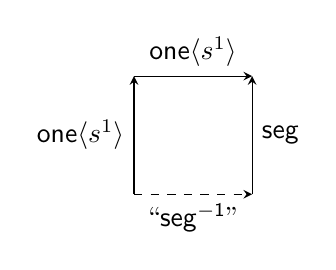
\begin{tikzpicture}[scale=.5]
    \draw[->,dashed,>=stealth] (0,0) -- (3,0) node [midway,below, fill=none] {``\cset{seg^{-1}}''};

    \draw[->,>=stealth] (0,3) -- (3,3) node [midway,above, fill=none] {\cont{\cset{one}}{\smap{1}}};
    \draw[->,>=stealth] (0,0) -- (0,3) node [midway,left, fill=none] {\cont{\cset{one}}{\smap{1}}};
    \draw[->,>=stealth] (3,0) -- (3,3) node [midway,right, fill=none] {\cset{seg}};
  \end{tikzpicture}
\end{center}

On the left and top side, the square is constantly \cset{one}. On the right hand
side, we have the \cset{seg} path. Then the bottom left corner of the square is
the 0-cell \cset{one} and the bottom right corner is \cset{zero}.
Kan composition of this open box gives us a cell with \cset{one} at its
left and \cset{zero} at its right boundary, which we could aptly call \cset{seg^{-1}}.

% TODO GOOD HERE?
% This principle has found its manifestation as a principle of logic. More general
% \cite{harper15_note_unifor_kan_condit_nomin_cubic_sets} by allowing multiple
% sides of the box to be missing and by also giving a filler for the whole cube,
% but this is not of concern for us in the following.

\todo{\cset{Int} is probably not the best motivating example. Can we find an example
  which feels very ``logicy'' and is not directly related to homotopy theory?}

\paragraph{Poset maps as interval substitutions}

The above examples are common proof obligations in Cubical Agda. Searching for
interval substitutions automatically is difficult since it is not possible to
construct a formula of the distributive lattice by looking at the boundary which
needs to be filled (at least according to the author's knowledge). We 
will have to take a different perspective in the following, using a
correspondence between $n$-tuples of formulas in the free bounded distributive
lattice over $m$ elements and monotone
functions between the posets  $\{ 0<1 \}^m$ and $\{ 0<1 \}^n$.

% This correspondence is efficiently computable as we will see in
% \ref{sec:cubicalcorrespondence}, where we flash out the correspondence between
% our presentation and the one in Cubical Agda more concretely.


For example, the formula $i \vee j$ corresponds to the poset map $\{ 0<1 \}^2
\to \{ 0<1 \}^1$ which sends $00$ to $0$ and everything else to $1$. In our
setting, a cubical set
is a presheaf on the full subcategory of posets of the form $\{ 0<1 \}^n$, which
means that this poset map will be sent contravariantly to a map from the 1-cells
to the 2-cells of the cubical set. By filling in the definition of \cset{seg}
for the 1-cell, we can depict the action of the poset map on the 1-cell
\cset{seg} as follows:
\begin{center}
\begin{tikzpicture}
  % \node (zz) at (0,1) {\textcolor{gray}{00} $\mapsto \{x\}$};
  % \node (zo) at (-1,0) {\textcolor{gray}{01} $\mapsto \{x , y\}$};
  % \node (oz) at (1,0) {\textcolor{gray}{10} $\mapsto \{x , y\}$};
  % \node (oo) at (0,-1) {\textcolor{gray}{11} $\mapsto \{y\}$};
  \node (zz) at (0,1) {00};
  \node (zo) at (-1,0) {01};
  \node (oz) at (1,0) {10};
  \node (oo) at (0,-1) {11};
  \draw (zz) -- (zo) -- (oo) -- (oz) -- (zz);
  % \end{tikzpicture}
  % \begin{tikzpicture}[scale=1]
  \node (z) at (2.6,.7) {\cset{zero}};
  \node (o) at (2.6,-.7) {\cset{one}};
  \draw (z) -- (o) node[midway,right] {\cset{seg}};

  \draw[|->] (zz) -- (z);
  \draw[|->] (zo) -- (o);
  \draw[|->] (oz) -- (o);
  \draw[|->] (oo) -- (o);
\end{tikzpicture}
\end{center}

This depiction suggests a geometrical intuition for how the boundary of $\lambda i
j.\cset{seg} (i \vee j)$ comes about: the faces $00-01$ and $00-10$ are the
\cset{seg} cell as $00$ is send to the left endpoint of \cset{seg} and $01$ and
$10$, respectively, to the right endpoint of \cset{seg}. The faces $01-11$ and $10-11$
are both constantly \cset{one} as both of its endpoints are send to the same
0-cell. This geometric intuition will allow us to find poset maps
efficiently, thereby solving the problem of finding interval substitutions in
TODO RUNTIME. This is a significant improvement over na\"ive search for
interval substitutions, as the number of $n$-dimensional interval substitutions of a
1-dimensional path is the $n$-th Dedekind number.

Moreover, the poset map perspective allows us to gradually build open box to
find cells as Kan compositions. The problem of whether a cell can be filled by
Kan composition is in general undecidable as we will show in
\autoref{ssec:kanundecidable}. We will explore different semi-decidable
procedures and heuristics to still come up with Kan compositions in many
practical examples.

% \cite{williamson12_combin_homot_theor}: we shall think geometrically, and prove
% algebraically!

% Allowable boundary shapes are generating cofibrations from a model categorical perspective



\paragraph*{Contributions and Structure}

The present paper is the first exploration of cubical sets from the point of
view of automated reasoning. We give a presentation of cubical sets in terms of
presheaves on a certain category of posets and monotone maps and give a notion
of normal forms for cells of cubical sets in \autoref{sec:normalforms}. We
introduce the notion of potential poset maps as a useful data structure for
efficient search of poset maps in \autoref{sec:contortionsolver} and give an
algorithm for finding poset maps for a given boundary with a run time of TODO RUNTIME.
We then extend our considerations to Kan cubical sets and establish why searching for
cells in Kan cubical sets is in general undecidable. We present efficient heuristics for
finding Kan compositions in many practical cases in
\autoref{sec:compositionsolver}. The findings of this paper have been used to
implement a tactic for Cubical Agda which we will discuss alongside some case studies in
\autoref{sec:cubicalagda} before concluding with some remarks in
\autoref{sec:conclusions}.


\section{Cubical Sets and Contortions}
\label{sec:normalforms}

In this section we will introduce the universe of discourse for our
considerations. We will define cubical sets and introduce some running examples
in \autoref{ssec:cubicalsets}. For proof search we require a finitary
representation of cubical sets, which we will call higher inductive types and
introduce in \autoref{ssec:hits}. We need a unique description for each cell of
a cubical set and introduce certain normal forms for this purpose in
\autoref{ssec:normalforms}.

\subsection{Cubical sets}
\label{ssec:cubicalsets}

The Dedekind cube category $\dedekind$ is the full subcategory of the category
of posets and monotone maps with objects $\pint{n}$ for $n \geq 0$, where $\pint{}
= \{ \izero < \ione \}$. Therefore morphisms in $\dedekind$ are of
the form $\pint{m} \to \pint{n}$. The cardinality of $\hom{\pint{m}}{\pint{}}$ is the
$m$-th Dedekind number, which explains the name of $\dedekind$.

We denote elements of $\pint{n}$ with $(e_1 \ldots e_n)$ where $e_i \in
\{\izero, \ione\}$ for $1 \leq i \leq n$ (we sometimes may omit the brackets).
For an element $x = (e_1 \ldots e_n)$ write $x_i \mdef e_i$. The poset
$\pint{0}$ has one element $()$. We will write $\pintrestr{n}{i}{e} \mdef
\{ x \in \pint{n} \mid x_i = e \}$, which is a subposet of $\pint{n}$.

% NECESSARY SOMEWHERE?
% Given $\pint{m} \to \pint{n}$ and a poset $P \subseteq \pint{m}$, we will denote
% with $\restrict{\sigma}{P} : P \to \pint{n}$ the restriction of $\sigma$ to $P$.
% In particular, if $P = \pintrestr{m}{i}{e}$, we might denote TODO INDEX REMOVED
% FROM IT

Cubical sets are objects of $\psh{\dedekind}$, i.e., presheaves over the
Dedekind cube category. For a cubical set $X$ write $X_n \mdef X(\pint{n})$,
which are called the $n$-cells of $X$. Given an element $p$ of $X_n$, we call
$\dim{p} \mdef n$ the dimension of $p$.

% If the cubical set $X$ is understood,
% write $\smap{i} \mdef X(s^i) : X_{n-1} \to X_n$ and $\dmap{i}{e} \mdef
% X(d^{(i,e)}) : X_n \to X_{n-1}$, these maps are called \mname{degeneracy maps}
% and \mname{face maps}, respectively.

Given an $n$-cell $p$, any poset map $\sigma : \pint{m} \to \pint{n}$ gives rise to an $m$-cell
$X(\sigma)(p)$. We will write $\cont{p}{\sigma} \mdef X(\sigma)(p)$ and call
$\cont{p}{\sigma}$ an $m$-contortion of $p$.

Certain poset maps of interest are:
\begin{align*}
  \smap{i} &: \pint{n} \to \pint{n-1}, (e_1 \ldots e_n) \mapsto (e_1 \ldots e_{i-1} e_{i+1} \ldots e_n) \text{ for } 1 \leq i \leq n\\
  \dmap{i}{e} &: \pint{n-1} \to \pint{n}, 
                (e_1 \ldots e_{n-1}) \mapsto (e_1 \ldots e_{i-1} e e_{i+1} \ldots e_{n-1}) \text{ for } 1 \leq i \leq n, e \in \{\izero,\ione\}
\end{align*}

Given an $n$-cell $p$, $\cont{p}{\smap{n+1}}$ is called a \mname{degeneracy} of
$p$. Given an $m > n$, we will write $\smap{m}$ for the composite
$\smap{n} \circ \smap{n+1} \circ \ldots \circ \smap{m}$. This gives the shorthand
$\cont{p}{\smap{m}}$ for $p$ considered as a degenerate $m$-cell.

Conversely, the cell $\cont{p}{\dmap{i}{e}}$ is called the $(i,e)$-th face of $p$. We
will call the list of all faces of an $n$-cell $p$ its boundary $\boundary{p}$:
$$\boundary{p} \mdef \mlist{ \cont{p}{\dmap{1}{\izero}},
  \cont{p}{\dmap{1}{\ione}} , \ldots , \cont{p}{\dmap{n}{\izero}}, \cont{p}{\dmap{n}{\ione}} }$$

% The functor laws of $X$ ensure that the faces of $p$ have overlapping
% boundaries. TODO GENERAL FORM

% Note that in any non-empty cubical set $X$, we must have non-empty $X_n$ for
% all $n$: given an $n$-cell $p$, the codomain $X_{n+1}$ of $\smap{n+1}$ as well
% as the codomain $X_{n-1}$ of $\dmap{n}{\_}$ must be non-empty.

% Not all poset maps can be obtained as compositions of degeneracy and face maps
% $s^\_$ and $d^\_$ (in contrast to simplicial sets).
% Therefore we will shift our attention to
% general poset maps $\sigma$ in the following.

Contravariance means that for an $n$-cell $p$, $\sigma : \pint{m} \to \pint{n}$ and $\tau : \pint{l} \to \pint{m}$ we have
$$\cont{\cont{p}{\sigma}}{\tau} = \cont{(\cont{p}{\sigma})}{\tau} = \cont{p}{\sigma \circ \tau}$$

% This means for instance
% $$\cont{\cont{p}{\sigma}}{\dmap{i}{e}} = \cont{p}{\restrict{\sigma}{\pintrestr{n}{i}{e}}}$$
% $$\dmap{i}{e}(X(\sigma)(p)) = X(\restrict{\sigma}{\pintrestr{n}{i}{e}})(p)$$


In this paper we will explore how one can come up with a cell given some
boundary. For this we will introduce some notation. An
$n$-dimensional boundary $T$ is a list of $2n$ cells $\mlist{p_{(1,\izero)},
  p_{(1,\ione)} , ... , p_{(n,\izero)}, p_{(n, \ione)}}$. We will write
$T_{(i=e)} \mdef p_{(i,e)}$. % TODO DO WE NEED THIS NOTATION


% In fact, we will be concerned in
% \autoref{sec:contortionsearch} with searching for intricate poset maps which
% give rise to cells with a specified boundary.


% A cubical set $X$ satisfies the Kan condition if for any open box
% $[t_1, s_1, \ldots , t_n , s_n] \ t$ we have a cell $s$ such that $[t_1,
% s_1, \ldots , t_n , s_n , t, s]$ is a valid boundary.\\[.5em]

% Call $\comp{[t_1, s_1, \ldots , t_n , s_n]}{t} \mdef s$

% When is a cubical set a \emph{type}, i.e., captures heterogenous identifications
% of elements in a type?

% Hope for syntax-free criterion.

% TODO Uniform Kan condition

% (still some issues: definitional equivalence of identity elimination has not
% been verified by model, only holds up to higher identification)
% A type is a cubical set satisfying the uniform Kan condition.

\begin{example}\label{exp:int}
  The cubical set $\cset{Int}$ is generated by the following data: $\cset{Int}_0
  = \{ \cset{zero} , \cset{one} \}$ and $\cset{seg} \in \cset{Int}_1$ with
  $\cont{\cset{seg}}{\dmap{1}{0}} = \cset{zero}$ and $\cont{\cset{seg}}{\dmap{1}{1}} =
  \cset{one}$, which we could have written more concisely with
  $\boundary{\cset{seg}} = \mlist{\cset{zero}, \cset{one}}$.

  $\cset{Int}$ contains all necessary contortions, for instance
  $\cont{\cset{zero}}{\smap{1}}$ is a well-defined 1-cell which is
  degenerately $\cset{zero}$.
  The identity map gives an $n$-contortion for every $n$-cell which is equal
  to the original cell, for instance $\cont{\cset{seg}}{\oneid}$ is just the cell
  $\cset{seg}$.

  % We have degenerate cells in higher dimensions for the $\smap{i}$
  % to have a codomain, for instance, $\smap{1}(\cset{zero})$ is a degenerate
  % 1-cell which is constantly $\cset{zero}$, captured by the fact that the face
  % maps $\dmap{1}{\_}$ send
  % $\smap{1}(\cset{zero})$ back to $\cset{zero}$.

  % Assuming that $\cset{Int}$ is Kan, we can obtain the reversal of $\cset{seg}$
  % as follows:
  % TODO Kan inversion example
\end{example}

\begin{example}\label{exp:sndsphere}
  We define the cubical set $\cset{Sphere}$ with the following data: We have a
  single 0-cell, so $\cset{Sphere}_0 = \{
  \cset{a} \}$. There is one non-degenerate 2-cell $\cset{\alpha} \in
  \cset{Sphere}_2$, which has a degenerate $\cset{a}$ for each of its faces,
  i.e.,
  $\boundary{\cset{\alpha}} = \mlist{ \cont{\cset{a}}{\smap{1}},
    \cont{\cset{a}}{\smap{1}}, \cont{\cset{a}}{\smap{1}}, \cont{\cset{a}}{\smap{1}} }$.
\end{example}

% \begin{example}\label{exp:torus}
%   We define the cubical set $\cset{Torus}$ with the following data: We have a
%   single 0-cell, so $\cset{Torus}_0 = \{ \cset{a} \}$. There are two
%   non-degenerate 1-cells $\cset{p}$ and $\cset{q}$ and one non-degenerate 2-cell
%   $\dmap{2}{0}(\cset{\alpha}) = \dmap{2}{1}(\cset{\alpha}) = p$ and
%   $\dmap{1}{0}(\cset{\alpha}) = \dmap{1}{1}(\cset{\alpha}) = q$.
% \end{example}

\begin{example}\label{exp:triangle}
  We define the cubical set $\cset{Triangle}$ as generated by the following
  data: The 0-cells are $\cset{Triangle}_0 = \{ \cset{x} , \cset{y} , \cset{z}
  \}$. The non-degenerate 1-cells are $\{ \cset{p} ,
  \cset{q} , \cset{r} \} \subseteq \cset{Triangle}_1$ with boundaries
  $\boundary{\cset{p}} = \mlist{ \cset{x} , \cset{y}}$
  $\boundary{\cset{q}} = \mlist{ \cset{y} , \cset{z}}$
  $\boundary{\cset{r}} = \mlist{ \cset{x} , \cset{z}}$.
  We have one non-degenerate 2-cell $\cset{\phi} \in \cset{Triangle}_2$ with
  $\boundary{\cset{\phi}} = \mlist{\cset{p} , \cset{r} , \cont{\cset{x}}{\smap{1}}  ,\cset{q}}$.
  

    % $\dmap{1}{0}(\cset{p}) = \cset{x}$ and $\dmap{1}{1}(\cset{p}) = \cset{y}$,
    % $\dmap{1}{0}(\cset{q}) = \cset{y}$ and $\dmap{1}{1}(\cset{q}) = \cset{z}$,
    % $\dmap{1}{0}(\cset{r}) = \cset{x}$ and $\dmap{1}{1}(\cset{r}) = \cset{z}$.
    % We have one non-degenerate 2-cell $\cset{\phi} \in \cset{Triangle}_2$ with $\dmap{1}{0}(\cset{\phi}) =
    % \cset{p}$, $\dmap{1}{1}(\cset{\phi}) = \cset{r}$, $\dmap{2}{0}(\cset{\phi})
    % = \smap{1}(\cset{x})$ and $\dmap{2}{1}(\cset{\phi}) = \cset{q}$.
\end{example}

% \begin{example}{\label{exp:assoc}}
%   Associativity of three paths
% \end{example}


\subsection{Higher inductive types}
\label{ssec:hits}

Cubical sets as introduced in the previous section are infinite objects:
as soon as there is a single cell in a cubical set $X$, we have faces or
degeneracies in all dimensions, and more generally all sorts of cells induced by
the poset maps. In order to mechanically search for cells in a cubical set, we
need a finitary representation of cubical sets. The examples above suggest that
we only require a bit of generating data from which the other cells and maps can
be inferred in a unique way.

% TODO BACKGROUND This is what HITs are for In
% \cite[Sect. 6.4]{bezem14_model_type_theor_cubic_sets}, strict groupoid turned
% into cubical set with general construction Higher inductive types are
% constructed as generalized pushout construction (free $\omega$-groupoid
% construction)


\begin{definition}
  A \mname{context} $\Gamma$ is a list of declarations $\mlist{ p_1 : T_1 ,
    \ldots , p_k : T_k}$. The cubical set $X$ generated by a context $\Gamma$
  has cells $p_i$ with boundaries $\boundary{p_i} = T_i$ for $1 \leq i \leq k$
  and all necessary other cells. We call $\ctxtdim{\Gamma} \mdef k$ the length
  of the context.
\end{definition}

\todo{Define validity of boundary and context descriptions and give algorithm
  checking validity.
  % Checking that a context is well-formed can be done in $\mathcal{O}(? k)$ and is
  % implemented in \autoref{alg:wellformedboundary} and
  % \autoref{alg:wellformedcontext}.
}

\begin{examplecontd}{exp:int}
  The following context generates $\cset{Int}$:
  
  $\mlist{ \cset{zero} : \mlist{} , \cset{one} : \mlist{} , \cset{seg} : \mlist{
      \cont{\cset{zero}}{}, \cont{\cset{one}}{} }}$
\end{examplecontd}

\begin{examplecontd}{exp:sndsphere}
  The following context generates $\cset{Sphere}$:

  $\mlist{ \cset{a} : \mlist{} , \cset{\alpha} : \mlist{ \cont{\cset{a}}{\oneconst} , \cont{\cset{a}}{\oneconst} ,
  \cont{\cset{a}}{\oneconst}, \cont{\cset{a}}{\oneconst} }}$
  
\end{examplecontd}

\begin{examplecontd}{exp:triangle}
  The following context generates $\cset{Triangle}$:
  
  % $\mlist{ \cset{x} : \mlist{} , \cset{y} : \mlist{} , \cset{z} : \mlist{} ,
  %     \cset{p} : \mlist{ \cont{\cset{x}}{}, \cont{\cset{y}}{} } ,
  %   , \cset{q} : \mlist{ \cont{\cset{y}}{}, \cont{\cset{z}}{} }
  %   , \cset{r} : \mlist{ \cont{\cset{x}}{}, \cont{\cset{z}}{} }
  %   , \cset{\phi} : \mlist{ \cont{\cset{p}}{\oneid} , \cont{\cset{r}}{\oneid} ,
  %     \cont{\cset{x}}{\oneconst}, \cont{\cset{q}}{\oneid} }
  % }$

  $\mlist{ \cset{x} : \mlist{} , \cset{y} : \mlist{} , \cset{z} : \mlist{} ,
    \cset{p} : \mlist{ \cset{x}, \cset{y}  } ,
    , \cset{q} : \mlist{ \cset{y}, \cset{z} }
    , \cset{r} : \mlist{ \cset{x}, \cset{z} }
    , \cset{\phi} : \mlist{ \cset{p} , \cset{r} ,
      \cont{\cset{x}}{\oneconst}, \cset{q} }
  }$

\end{examplecontd}



In the following we will assume a valid context $\Gamma$
generating a cubical set $X$.


\subsection{Normal forms of contortions}
\label{ssec:normalforms}

There are different ways of describing a cell in a cubical set.
For our
considerations we will want a unique representation for every cell to allow for
literal comparisons between cells.
For instance in \autoref{exp:int}, both $\cont{\cset{zero}}{\oneconst}$ and
$\cont{\cset{seg}}{\substtwo{0}{0}}$ describe the same cell, namely the degenerate
1-cell which is constantly $\cset{zero}$. Since the former has a lower dimension, 
we will regard it as the normal form of this cell. In general:

\begin{definition}
  A contortion $\cont{p}{\sigma}$ is in normal form if there is no face $q$ of
  $p$ and map $\tau$ such that $\cont{p}{\sigma} = \cont{q}{\tau}$.
\end{definition}

We can efficiently compute the normal form of a contortion with
\autoref{alg:normalize}. Given a contortion $\cont{p}{\sigma}$,
we check whether $\sigma$ sends all elements of $\pint{m}$ to a
subposet $\pintrestr{n}{i}{e}$ of $\pint{n}$, which means that the contortion in
fact only talks about a face of $p$. If this is not the case we already
have been given a normal
form. Otherwise, we retrieve the $(i,e)$-th face of $p$, which we call $q$, and
normalize $q$ with the composed contortion.


\begin{algorithm}[H]
  \caption{Normalizing a contortion}
  \label{alg:normalize}
  \begin{algorithmic}
    \Require $\cont{p}{\sigma}$ where $p : T \in \Gamma$ is an $n$-cell and
    $\sigma : \pint{m} \to \pint{n}$ \Ensure Normal form of $\cont{p}{\sigma}$

    \Procedure{Normalize}{$\cont{p}{\sigma}$}
    \If{$\exists 1 \leq i \leq n, e
      \in \{\izero, \ione\} : \image{\sigma} \subseteq \pintrestr{n}{i}{e}$}
    \State $\cont{q}{\tau} \gets \cont{p}{\dmap{i}{e}}$
    \State \Return{$\Call{Normalize}{\cont{q}{\tau \circ s^i \circ \sigma }}$ }
    \Else{}
    \State \Return{$\cont{p}{\sigma}$}
    \EndIf
    \EndProcedure

  \end{algorithmic}
\end{algorithm}

The algorithm is correct by the following reasoning: For a poset map $\sigma :
\pint{m} \to \pint{n}$ which satisfies for some $1 \leq i \leq n$, $e \in
\{\izero, \ione\}$ that $\sigma(x)_i = e$ for all $x \in \pint{m}$, we naturally
have $\sigma = \dmap{i}{e} \circ \smap{i} \circ \sigma$.
But then we have by functoriality for $\cont{q}{\tau} \mdef \cont{p}{\dmap{i}{e}}$:
$$\cont{p}{\sigma} = \cont{p}{\dmap{i}{e} \circ \smap{i} \circ \sigma} =
\cont{\cont{p}{\dmap{i}{e}}}{\smap{i} \circ \sigma} =
\cont{\cont{q}{\tau}}{\smap{i} \circ \sigma} = \cont{q}{\tau \circ \smap{i} \circ \sigma}$$

% This map comes about as follows: we
% know that  $\sigma(x)_i$ is the same for all $x \in \pint{m}$, so we can obtain
% $\cont{p}{\sigma}$ also as a contortion of $q$ by first applying $\sigma$, then
% forgetting about index $i$ with $s^i$ and finally applying the contortion
% of the face, $\sigma'$.

If we compute $\image{\sigma}$ as a multiset, checking whether 
$\image{\sigma}$ only contains elements of $\pintrestr{n}{i}{e}$ for
some $1 \leq i \leq n$ and $e \in \{\izero,\ione\}$ takes $\mathcal{O}(2^mn)$
(go through all $n$ indices of all $2^m$ elements of $\image{\pint{m}}$ and
return the first index at which all elements are the same, if there is such an index).
Since the dimension of the contortion under question is decreased by 1 in each
normalization step, we need to run the algorithm at most $n$ times and therefore
have a total complexity of $\mathcal{O}(2^mn^2)$ for contortion normalization.

\begin{examplecontd}{exp:triangle}
  The contortion $\cont{\phi}{\substfour{00}{00}{01}{01}}$ has normal form $\cont{p}{\substfour{0}{0}{1}{1}}$.
\end{examplecontd}

More results: for normal forms we do not have to worry about poset maps

\begin{proposition}
  Uniqueness of contortions: if $\boundary{\cont{p}{\sigma}} =
  \boundary{\cont{p}{\tau}}$ TODO ABOVE WITHOUT boundary, then $\sigma = \tau$.

  \begin{proof}
    \todo{As soon as poset map differs in one point, then completely different
      boundary??? Proof by contradiction? Or counting argument?}
  \end{proof}
\end{proposition}


This lemma will be relevant when searching for contortions:

\begin{proposition}
  If $\cont{p}{\sigma}$ is in normal form for $\dim{p} = n$ and $\sigma :
  \pint{m} \to \pint{n}$ with $m > n$, then there is a face $\cont{p}{\tau}$ of
  $\cont{p}{\sigma}$ (with $\tau : \pint{m-1} \to \pint{n}$).

  \begin{proposition}
    \todo{For $m=n$ this does not hold: fgfg square filled with triangle. For
      $m>n$ I wasn't able to construct a cube containing f and g but not the
      triangle. Check with brute force this really does not hold?}
  \end{proof}
  
\end{proposition}

This means that if we are given a boundary of a cell, we do not have to check
all faces: todo which not.

Furthermore, we can use this cell to reduce the search space.



% \todo{where to describe \autoref{alg:boundary} }

% TERM DEFINITION 
% Given a context $\Gamma$, the set of $m$-dimensional terms over $\Gamma$, denoted $Tm_m(\Gamma)$, consists of
% \begin{itemize}
% \item Contortions $\cont{p}{\sigma}$ with $p \in \Gamma$ and $\sigma : \pint{m} \to
%   \pint{\dim{p}}$
%   % \item Kan compositions, i.e., $\comp{[(t_1 , s_1) , (t_m, s_m)]}{t}$ for all
% \item Kan compositions, i.e., $\comp{[t_1 , s_1, ... , t_m, s_m]}{t}$ for all
%   fitting $m$-contortions $t_1 , s_1, ... , t_m, s_m, t$.
% \end{itemize}


\section{Searching for Contortions}
\label{sec:contortionsolver}

In this section, we will study the following search problem: given a cubical set
and a certain boundary, we want to decide whether there is a cell in this
cubical set with that boundary. We will set out this problem in more detail in
\autoref{ssec:cubicalcell}. For our algorithms we introduce the notion of
potential poset maps which are introduced in \autoref{ssec:ppm} and use them to
devise an efficient algorithm for computing contortions in
\autoref{ssec:contortionsolver}. 


\subsection{The problem \myproblem{CubicalCell}}
\label{ssec:cubicalcell}

Using the finitary representation introduced above, we can phrase the problem of
finding a cell with a given boundary as follows:

\begin{definition}
  Given a context $\Gamma$ and a boundary $T$, the problem
  \myproblem{CubicalCell}($\Gamma$,$T$) is to find a contortion $\cont{p}{\sigma}$ such that
  $\boundary{\cont{p}{\sigma}} = T$.
\end{definition}

The problem \myproblem{CubicalCell} is clearly decidable since there are
only finitely many contortions of a cell in a specific dimension. However, the
search space grows super-exponentially: suppose we want to find an
$m$-dimensional contortion of a 1-cell, i.e., we are looking for a poset map
$\pint{m} \to \pint{}$. The number of such monotone maps is the $m$-th Dedekind
number, which we will denote $D_m$. For $m = 6$, we already have $D_6 = 7828354$
poset maps, and for 9 the exact number of possible poset maps is unknown
\footnote{\url{http://oeis.org/A00372}}. The number of such poset maps grows
furthermore exponentially with the dimension of the path that is contorted,
i.e., we have $D_m^n$ many monotone maps $\pint{m} \to \pint{n}$. 
Therefore bruteforcing the search for contortions gets quickly infeasible and we
require something more clever to explore the search space.

% A certainly decidable subproblem of \myproblem{CubicalCell} is to decide whether
% there exists a cell simply by means of contorting the cells given in the
% context: for a given goal boundary $T$ and a generating cell $p$, there are
% finitely many poset maps $\pint{\dim{T}} \to \pint{\dim{p}}$, so we can
% na\"ively check whether one of those maps gives rise to a fitting contortion. 

% We can try this for all elements in the context, thereby have run time
% $\mathcal{O}( \ctxtdim{\Gamma} )$



% \subsection{General complexity considerations}
% Revert characterization 
% $$\dmap{i}{e}(X(\sigma)(p)) = X(\restrict{\sigma}{\pintrestr{n}{i}{e}})(p)$$
% TODO WHAT DID I MEAN BY THIS


\subsection{Potential poset maps}
\label{ssec:ppm}

For the following algorithms we introduce the notion of a potential poset map. In
essence, a potential poset map keeps track of all the potential values that elements of
the domain of the poset map might have, while making sure that there are no
superfluous values that cannot be part of any poset map as they would otherwise
violate monotonicity. Thereby we can represent all maps $\pint{m} \to \pint{n}$
at once with little data.

\begin{definition}
  % A \mname{potential poset map} (\mname{ppm}) is a map $\Sigma : \pint{m} \to \pow{\pint{n}}$
  % such that for all $x \leq y$ : for all $u \in \Sigma(x)$ exists $v \in
  % \Sigma(y)$ such that $u \leq v$. TODO MORE

  A \mname{potential poset map} (\mname{ppm}) is a map $\Sigma : \pint{m} \to \pow{\pint{n}}$
  such that $\forall x \leq y$:
  \begin{itemize}
  \item $\forall u \in \Sigma(y) : \exists v \in \Sigma(x) : v \leq u$.
  \item $\forall v \in \Sigma(x) : \exists u \in \Sigma(y) : v \leq u$.
  \end{itemize}

\end{definition}

The two conditions above mean that any possible value in a ppm will give
rise to at least one poset map.
We will represent ppms simply with their graphs. We also
list the vertices such that if $x \leq y$ then $x$ is earlier than $y$ in the
list. This allows us to traverse through the graph and know that if an element
$x$ is at a certain position in the list, all elements below $x$ will be seen at
a certain point.

We will extend the notion of a contortion as a poset map applied to a cell to
also incorporate potential poset maps, leading to the notion of potential contortions.

\begin{examplecontd}{exp:int}
  We have the following potential contortion
  $\cont{\cset{seg}}{\substfour{\{0\}}{\{0, 1\}}{\{0, 1\}}{\{1\}}}$. To
  understand its action in the cubical set \cset{Int} we again fill in the
  definition of \cset{seg} into the poset map as follows:

  \begin{center}
      \begin{tikzpicture} %scale=1.3]
        % \node (zz) at (0,1) {\textcolor{gray}{00} $\mapsto \{x\}$};
        % \node (zo) at (-1,0) {\textcolor{gray}{01} $\mapsto \{x , y\}$};
        % \node (oz) at (1,0) {\textcolor{gray}{10} $\mapsto \{x , y\}$};
        % \node (oo) at (0,-1) {\textcolor{gray}{11} $\mapsto \{y\}$};
        \node (zz) at (0,1) {\textcolor{gray}{00}};
        \node (zo) at (-1,0) {\textcolor{gray}{01}};
        \node (oz) at (1,0) {\textcolor{gray}{10}};
        \node (oo) at (0,-1) {\textcolor{gray}{11}};
        \draw (zz) -- (zo) -- (oo) -- (oz) -- (zz);
        % \end{tikzpicture}
        % \begin{tikzpicture}[scale=1]
          \node (z) at (2.6,.7) {\cset{zero}};
          \node (o) at (2.6,-.7) {\cset{one}};
          \draw (z) -- (o) node[midway,right] {\cset{seg}};

          \draw[|->] (zz) -- (z);
          \draw[|->] (zo) -- (z);
          \draw[|->] (zo) -- (o);
          \draw[|->] (oz) -- (o);
          \draw[|->] (oz) -- (z);
          \draw[|->] (oo) -- (o);
      \end{tikzpicture}
    \end{center}

  % \vspace{1em}
      The ppm can be unfolded into four poset maps as we can choose the values
      of $01$ and $10$ independently. The squares resulting from using these
      poset maps for contortions of \cset{seg} are depicted below:

      \filledsquare{\cset{seg}}{\cset{seg}}{}{}{\substfour{0}{0}{1}{1}}
      \filledsquare{\phantom{\cset{seg}}}{\phantom{\cset{seg}}}{\cset{seg}}{\cset{seg}}{\substfour{0}{1}{0}{1}}
      \filledsquare{\cset{seg}}{\phantom{\cset{seg}}}{\cset{seg}}{}{\substfour{0}{1}{1}{1}}
      \filledsquare{\phantom{\cset{seg}}}{\cset{seg}}{}{\cset{seg}}{\substfour{0}{0}{0}{1}}

      All these contortions have in common that the bottom left corner is
      \cset{zero} and the top right corner is \cset{one}, which we could already
      read off from the potential contortion.

\end{examplecontd}

Thereby ppms are a very useful notion to capture a number of poset maps with
little data. For example, representing all $D_n$ poset maps $\pint{n} \to
\pint{}$ requires only $2^n$ entries of $\{0,1\}$. Our goal in the following
will be to restrict a ppm until only few poset maps remain. We can unfold a ppm
into the set of poset maps that it is representing with
\autoref{alg:getsubsts} given in the appendix. We can restrict the values of a
ppm with \autoref{alg:updateppm}. % me of 
% From a potential poset map we can generate all poset maps. This has a worst-case
% runtime of Dedekind for the full one.

A non-empty ppm is one which has a non-empty set of possible values
for any element, which can be checked in $2^m$ steps. Given a poset $xs
\subseteq \pint{m}$, we can restrict a ppm $\Sigma : \pint{m} \to \pow{\pint{n}}$ to a
new ppm $\restrict{\Sigma}{xs} : xs \to \pow{\pint{n}}$ just like any function.


\subsection{Contortion solver}
\label{ssec:contortionsolver}

Using the notion of potential poset maps, we give the following algorithm to
generate a contortion for a given boundary.

\begin{algorithm}[H]
  \caption{Contortion solver}\label{alg:simple}
  \begin{algorithmic}
    \Require $\Gamma$ context, $p \in \Gamma$, $T$ goal boundary with $n \mdef \dim{p} , m \mdef \dim{T} $
    \Ensure $\sigma$ s.t. $\boundary{\cont{p}{\sigma}} = T$ if there is such a
    $\sigma$, \texttt{Unsolvable} otherwise

    \Procedure{ContortionSolve}{$p$} % TODO WHICH INPUT
    \State $\Sigma \gets \{ x \mapsto \pint{n} \mid x \in \pint{m} \}$
    \For{$\cont{q}{\tau} \mdef T_{i=e} \text{ with } i \gets 1\leq i \leq m, e \gets \{\izero,
      \ione\}, \dim{q} $ desc.}
    % \For{$i \gets 1\leq i \leq m, e \gets \{\izero, \ione\}$}
    \If{$p = q$}
      \State $\Theta \gets \{ x \mapsto \tau(x) \mid x \in \pintrestr{m}{i}{e} \}$
    \Else
      \State $\Theta \gets \{ x \mapsto \emptyset \mid x \in \pintrestr{m}{i}{e} \}$
      \For{$\sigma \gets \Call{UnfoldPPM}{\restrict{\Sigma}{\pintrestr{m}{i}{e}}}$}
        \If{$T_{i=e} = \Call{Normalize}{\cont{p}{\sigma}}$}
          \For{$x \in \pintrestr{m}{i}{e}$}
            \State $\Theta(x) \gets \Theta(x) \cup \{ \sigma(x) \}$
          \EndFor
        \EndIf
        \EndFor
        \EndIf
      \For{$x \in \pintrestr{m}{i}{e}$}
      \State \Call{UpdatePPM}{$\Sigma, x, \Theta(x)$}
      \EndFor
    \EndFor
    \If{$\exists \sigma \in \Call{UnfoldPPM}{\Sigma} : \boundary{\cont{p}{\sigma}} = T$}
      \State \Return{$\sigma $}
    \Else
    \State \Return{\texttt{Unsolvable}}
    \EndIf
    \EndProcedure
  \end{algorithmic}
\end{algorithm}

The idea of the algorithm is as follows: We first generate the most general ppm
$\Sigma$. We then go through each face $\cont{q}{\tau}$ of the goal boundary $T$
and use it to restrict $\Sigma$. Crucially, we order the faces by their
dimensions as higher-dimensional faces in the boundary will restrict $\Sigma$
more than lower-dimensional faces. In the most extreme case, $q$ will have the
same dimension as $p$, which allows us to give a unique value for each element
of the face $q$, i.e., each element of $\pintrestr{m}{i}{e}$ if $\cont{q}{\tau}$ was
the $(i,e)$-th face. Otherwise, we will check for each element of $\pintrestr{m}{i}{e}$ which
values lead to some contortion which is equal to $\cont{q}{\tau}$. To do this we
need to unfold $\Sigma$ at this subposet and check for each resulting poset map
if it gives rise to a valid contortion.

The algorithm is obviously correct since we only return a poset map $\sigma$ if
it is indeed contorting $p$ to the correct boundary.

\todo{It appears that we do not need this filter! Can we prove this?}

% Instead of having to check all $D_m^n$ poset maps, we have to check in the worst
% case $2 m D_{m-1}^n$ poset mapos.

% \begin{algorithm}[H]
%   \caption{Simple solver recursively}\label{alg:simple}
%   \begin{algorithmic}
%     \Require $\Gamma$ context, $p \in \Gamma$, $T$ goal boundary ($n \mdef \dim{p} , m \mdef \dim{T} $)
%     \Ensure All $\sigma$ s.t. $\boundary{\cont{p}{\sigma}} = T$

%     \Procedure{SimpleSolve}{$p$}
%     \State $\Sigma \gets \{ x \mapsto \pint{n} \mid x \in \pint{m} \}$
%     \For{$i \gets 1\leq i \leq m, e \gets \{\izero, \ione\}$}
%       \State $\Theta \gets (x : \pintrestr{m}{i}{e} )\mapsto \emptyset$
%       \For{$\sigma \gets \Call{SimpleSolve}{\boundary{T_{i=e}}}$}
%         \For{$x \in \pintrestr{m}{i}{e}$}
%           \State $\Theta(x) \gets \Theta(x) \cup \{ \sigma(x) \}$
%         \EndFor
%         \EndFor
%         \For{$x \in \pintrestr{m}{i}{e}$}
%           \State \Call{UpdatePPM}{$\Sigma, x, \Theta(x)$}
%         \EndFor
%     \EndFor
%     \State \Return{$\{ \sigma \mid \sigma \in \Call{UnfoldPPM}{\Sigma} :
%     \boundary{\cont{p}{\sigma}} = T \}$}
%     \EndProcedure
%   \end{algorithmic}
% \end{algorithm}


% More than that, the potential substitutions allow us to narrow down the search
% space in other ways.

% Try to reduce the search space going from the bottom.


\todo{Prove completeness of \autoref{alg:simple}. This is not essentially difficult to
  see, but requires some reasoning.}

\todo{Prove run time of \autoref{alg:simple}. I have not been able to come up
  with an argument for this. Potentially, unfolding the subposet corresponding
  to a face could lead to $D_{m-1}^n$ many poset maps which need to be checked,
  hence we would only reduce the complexity to the previous Dedekind number.
  However, in all examples I have encountered we have one face $q$ which is the
  same as $p$, therefore we can significantly reduce the size of $\Sigma$ before
we need to do any unfolding. I do not yet know if this is always the case and
what this means for the worst-case complexity of the algorithm. }


\begin{examplecontd}{exp:sndsphere}

  We will now sketch an example run of \autoref{alg:simple}. We want to find a
  $\sigma : \pint{3} \to \pint{2}$ such that $\cont{\alpha}{\sigma}$ has this boundary:
$$\mlist{ \cont{\cset{\alpha}}{\substfour{00}{01}{01}{11}} ,
  \cont{\cset{a}}{\smap{2}} , \cont{\cset{a}}{\smap{2}} ,
  \cont{\cset{a}}{\smap{2}} , \cont{\cset{a}}{\smap{2}} ,
  \cont{\cset{a}}{\smap{2}}}$$

In the beginning, the ppm $\Sigma$ is initialized totally with $\{ x \mapsto
\pint{2} \mid x \in \pint{3}\}$.

We then go through all faces of the goal boundary and use them to restrict
$\Sigma$.
The first face of the boundary is a contortion of $\alpha$, which is the
highest-dimensional face, so we use it to restrict $\Sigma$. Since $\alpha$ is also
the cell that we are contorting, the subposet $\pintrestr{3}{1}{\izero}$
of the domain of $\Sigma$
is mapped in a unique way to the elements of $\pint{2}$. The monotonicity
restrictions on ppms further restrict $\Sigma$: since $011$ is mapped to the
bottom element $00$, also $111$ will need to be mapped to $00$. The elements
$101$ and $110$ lie below elements which are mapped to $01$, which mean that
there are only two possible values $\{01, 11\}$ for each of these elements. Only
the element $001$ has the full poset $\pint{2}$ as potential values. In summary,
we have the following potential contortion after the first restriction of $\Sigma$:

\begin{center}
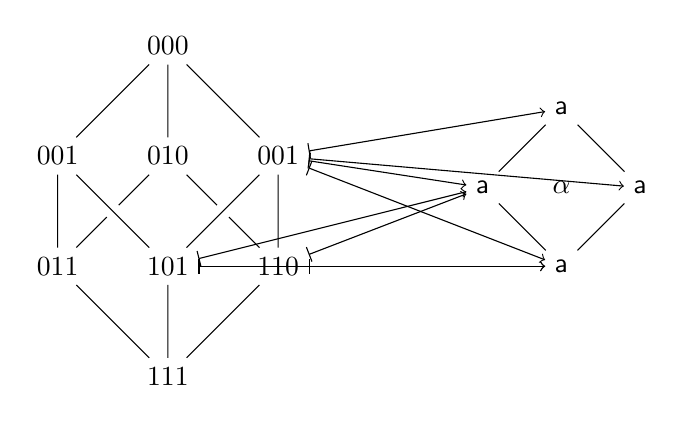
\begin{tikzpicture}
      \node (zzz) at (0,2.8) {$000$};
      \node (zzo) at (-1.4,1.4) {$001$};
      \node (zoz) at (0,1.4) {$010$};
      \node (zoo) at (-1.4,0) {$011$};
    \node (ozz) at (1.4,1.4) {$001$};
    \node (ozo) at (0,0) {$101$};
    \node (ooz) at (1.4,0) {$110$};
    \node (ooo) at (0,-1.4) {$111$};
    \draw (ooo) -- (zoo) -- (zzo) -- (zzz) -- (zoz) -- (ooz)
    (ozo) -- (ooo) -- (ooz) -- (ozz) -- (zzz)
    (zoo) -- (zoz);
    \draw[preaction={draw=white, -,line width=6pt}] (zzo) -- (ozo) -- (ozz);

    \begin{scope}[shift={(5,1)}]
      \node (zz) at (0,1) {\cset{a}};
      \node (zo) at (-1,0) {\cset{a}};
      \node (oz) at (1,0) {\cset{a}};
      \node (oo) at (0,-1) {\cset{a}};
      \node (filler) at (0,0) {\cset{\alpha}};
      \draw (zz) -- (zo) -- (oo) -- (oz) -- (zz);
    \end{scope}

    \draw[|->] (ozo) -- (zo);
    \draw[|->] (ozo) -- (oo);
    \draw[|->] (ooz) -- (zo);
    \draw[|->] (ooz) -- (oo);
    \draw[|->] (ozz) -- (zz);
    \draw[|->] (ozz) -- (zo);
    \draw[|->] (ozz) -- (oz);
    \draw[|->] (ozz) -- (oo);
  \end{tikzpicture}
\end{center}

We then check for each of the faces which are degenerate \cset{a} whether
$\Sigma$ gives rise to such a face. Crucially, this will be done quickly as
there are only 10 poset maps in the ppm $\Sigma$ remaining after the reduction
of $\Sigma$ with the first face.

\end{examplecontd}


% \begin{examplecontd}{exp:sndsphere}
%   TODO UPDATE WITH NEW ALGORITHM
%   5-dimensional analogue of above cube is solved in  $< 5$ seconds.
%   Try out $\mathcal{O}(D_4^2 = 168^2 = 28224)$ poset maps for all 10 faces, combine all
%   fitting poset maps in ppm.
%   This ppm unfolds to 168 poset maps of type
%   $\pint{5} \to \pint{2}$, filter which one fits.

%   Brute force approach would require checking $D_5^2 = 7581^2 = 57,471,561$
%   poset maps.
% \end{examplecontd}






\section{Composition solver}
\label{sec:compositionsolver}

\todo{This section only exists as a rough scaffolding.}

\subsection{Kan cubical sets}

A cubical set $X$ satisfies the Kan condition if for any open box
$[t_1, s_1, \ldots , t_n , s_n] \ t$ we have a cell $s$ such that $[t_1,
s_1, \ldots , t_n , s_n , t, s]$ is a valid boundary. Call $\comp{[t_1, s_1,
  \ldots , t_n , s_n]}{t} \mdef s$ the Kan composition of the box. 

\todo{Make more general to uniform Kan condition}

\begin{definition}
  Given a context $\Gamma$ and a (valid) boundary $T$, the problem
  \myproblem{KanCubicalCell}($X$,$T$) is to find an open box $[t_1, s_1, \ldots ,
  t_n , s_n] \ t$ such that $\boundary{\comp{[t_1, s_1, \ldots , t_n , s_n]}{t}} = T$.
\end{definition}



\subsection{Undecidability of finding Kan compositions}
\label{ssec:kanundecidable}

Since Kan cubical sets are a model of groupoids and groupoids are a generalization
of groups, it is no surprise that we can encode groups with cubical sets.
Since also Kan composition is sufficient to generate concatenations of paths
etc, we can encode word problems for groups, which can be used to show that ..
is undecidable.
 

\begin{theorem}
  \myproblem{KanCubicalCell} is undecidable.
  \begin{proof} 
    We show how the word problem for groups \myproblem{WordGroup} reduces to
    \myproblem{KanCubicalCell}.

    Given a finitely generated group $G = \langle X \mid R \rangle$ with neutral
    element $e$ and where $X$ are its set of generators and $R$ relations over
    $X$, i.e., $R \subseteq \{ a_1 \mathellipsis a_n \mid a_\_ \in X \cup X^{-1}
    \}$ such that for all $w \in R$, we have $w = e$ in $G$.
    

    Construct the cubical set \cset{G} with 0-cell $\star$, 1-cells $X$ with
    $\boundary{p} = \mlist{\star , \star}$ for any $p \in X$, and for each $w \
    \in R$ a 2-cell $r_w$ with $\boundary{r_w} = \mlist{ w , \cont{\star}{\smap{1}} ,
      \cont{\star}{\smap{1}} , \cont{\star}{\smap{1}}}$ where $w$ is the
    composition of words

    \todo{We need to have introduced compositions as this point}
    \todo{We need to have introduced inverses as this point}

    Given a word $v$ in $G$, we now want to decide whether $v = e$ in $G$.
    Suppose that \myproblem{KanCubicalCell} was decidable. We show that we can
    then decide \myproblem{WordGroup}

    Given $s$ = Comp such that $\boundary{s} = \mlist{ v , ... }$
    
    % Finitely generated: $X$ is finite
    % Finitely presented: $X$ and $R$ are finite
    
    Suppose $R$ infinite or something?

    % Given a set of generators $\{a, ...\}$ of a group $G$, define $\cset{Group}$
    % with a single 0-cell $\cset{Group}_0 = \{ \cset{\star} \}$, 
    % 1-cells $\{\cset{a} , \cset{a^{-1}} ... \} \subseteq \cset{Group}_1$ and a
    % 2-cell $\cset{idem_a}$ for any generator $a$ with 
    % $\dmap{2}{0}(\cset{idem_a}) = \cset{a}$, $\dmap{1}{1}(\cset{idem_a}) =
    % \cset{a^{-1}}$ and $\dmap{2}{1}(\cset{idem_a}) = \dmap{1}{0}(\cset{idem_a}) = \smap{1} (\cset{\star})$.

    % Given a set of generators $\{a, ...\}$ of a group $G$, define $\cset{Group}$
    % with a single 0-cell $\cset{Group}_0 = \{ \cset{\star} \}$, 
    % 1-cells $\{\cset{a} , ... \} \subseteq \cset{Group}_1$ 

    % (there are more 2-cells that need to be added as explained in \cite[Sect. 6.3]{bezem14_model_type_theor_cubic_sets})
    % % Note that this is not a set. Doesn't matter for undecidability proof?

    \todo{Give reduction Word < KanCubicalCell. For some specific group with
      undecidable word problem or Uniform word problem? }
\end{proof}
\end{theorem}


\subsection{A semi-deciability procedure for 1-dimensional cubes}

\todo{Only going in one side direction will always yield a proof, if it exists}

\subsection{Decidability of finitely generated groups}

\todo{Carry over some decidability results from the word problem for groups over
to our setting?}


% \section{Negation}

% How to encode search for reversals


\section{A Tactic for Cubical Agda}
\label{sec:cubicalagda}

We have reasoned about semantic objects in this paper: since syntax and semantics so
closely linked, this gives us a syntactic solver as well. We just have to
translate to the term language of Cubical Agda.

The above algorithms have been implemented in
\url{https://github.com/maxdore/cubetac/}. In the following we will discuss how
our approach relates to Cubical Agda and a case study using this tactic.


% As observed by \cite{orton17_axiom_model_cubic_type_theor_topos}, we do not require
% a full De Morgan structure. In particular, it suffices to consider only $\meet$
% and $\join$ forming a bounded free distributive lattice. Model structure open
% problem, but it is conjectured that it does.


\subsection{Translating to Cubical Agda}

The morphisms in $\dedekind$ have a succinct description as tuples of formulas
of a free distributive lattices, these formulas are also used in Cubical Agda.
In order to use our algorithms in a tactic for Cubical Agda, we need to
translate back and forth efficiently between both characterizations of $\dedekind$.

To generate a lattice formula from a poset map we can use \autoref{alg:subst2tele}.

\begin{algorithm}[H]
  \caption{Poset map to lattice formula}\label{alg:subst2tele}
  \begin{algorithmic}
    \Require $\sigma : \pint{m} \to \pint{n}$
    \Ensure $\phi$ $n$-tuple of elements of free distributive lattice over $m$ variables

    \Procedure{Subst2Tele}{$\sigma$}
    \For{$i \gets 1$ to $n$} 
      \State $\phi_i \gets \{ x \in \pint{m} \mid \sigma(x)_i = 1 \}$
      \Comment{$\mathcal{O}(2^m)$ many elements in $\pint{m}$}
    \EndFor
    \State \Return{$(\phi_1, ... , \phi_n)$}
    \EndProcedure
  \end{algorithmic}
\end{algorithm}

Given $\sigma : \pint{m} \to \pint{n}$, we compute an $n$-tuple of elements of the
free distributive lattice over $m$ elements as follows:
The $i$-th entry is $\{ x \in \pint{m} \mid s(x)_i = 1 \}$. An element $x$ can be
seen as a clause if we regard it as indicator of which elements of the lattice
are used, e.g., $(1,0,1)$ represents the clause $x \meet z$ if the three
elements of the lattice are $x$, $y$ and $z$.

% TODO mention set representation of DNF. Also mention normalization necessary --
% what's its runtime?

For the converse we can use \autoref{alg:teletosubst}

\begin{algorithm}[H]
  \caption{Lattice formula to poset map}\label{alg:teletosubst}
  \begin{algorithmic}
    \Require $\phi$ $n$-tuple of elements of free distributive lattice over $m$ variables
    \Ensure $\sigma : \pint{m} \to \pint{n}$

    \Procedure{Tele2Subst}{$p$}
    \For{$x \gets \pint{m}$} 
      \For{$i \gets 1$ to $n$}
        \State $\sigma(x)_i \gets \phi_i @ x$
      \EndFor
    \EndFor
    \State \Return{$\sigma$}
    \EndProcedure
  \end{algorithmic}
\end{algorithm}

From an $n$-tuple of formulas over $\phi$ we can read off a poset map $\sigma :
\pint{m} \to \pint{n}$ as follows: Given an element $x \in \pint{m}$, $\sigma(x) = (e_1
, ... , e_n) $ where $e_i = \phi_i @ x$. Here $\phi_i$ is the $i$-th element of
the tuple $\phi$ and $@$ denotes evaluation of formulas: The indices of $x$
which are set to 1 mean that the corresponding variable of $\phi$ is ``true'',
then we check whether the formula evaluates in total to true by interpreting
join and meet as logical operations.

\todo{The above presentation is not very clean and should be streamlined.}

Therefore going back and forth between formulas and poset map takes
$\mathcal{O}(2^mn)$ many steps. This is linear in the number of elements of the
data structures we are considering, so does not pose an issue for performance of
our tactic.

% \begin{example}
%   % EXAMPLE
%   % [(000,00),(001,00),(010,00),(011,01),(100,10),(101,11),(110,10),(111,11)]
%   % 1 ((2 /\ 3) \/ (1 /\ 3))
% \end{example}

% TODO PROOF THAT THESE ARE MUTUALLY INVERSE?
\todo{Show correctness of both algorithms and that they are mutually inverse.}

\subsection{Translating to PathP types}

Cubical Agda uses PathP types to represent boundaries of a cube. The PathP type
has three constructors, where the first is again a PathP type, allowing for
nesting paths and thereby creating higher cubes. If the second and third
parameter are $n$-dimensional paths, then the first parameter might introduce
$n$ interval variables.


\begin{examplecontd}{exp:sndsphere}
  
The proof goal already introduced above:

$$\mlist{ \cont{\cset{p}}{\substfour{00}{01}{01}{11}} ,
  \cont{\cset{a}}{\smap{2}} , \cont{\cset{a}}{\smap{2}} ,
  \cont{\cset{a}}{\smap{2}} , \cont{\cset{a}}{\smap{2}} ,
  \cont{\cset{a}}{\smap{2}}}$$

has the following corresponding PathP type in Cubical Agda.
  \begin{align*}
    \mathsf{PathP} (\lambda i \to \mathsf{PathP} &(\lambda j \to  \mathsf{Path} \ (\cset{p} \ (i \wedge
                                                   j) \ (i \vee j))\ \cset{a})\\
                                                 &(\lambda j \to \cset{a}) (\lambda j \to \cset{a}))
                                                   (\lambda i j \to \cset{a}) (\lambda i j \to \cset{a})
  \end{align*}
\end{examplecontd}

\todo{Translating between our notions and PathP types is straightforward, we
  should still explain it here}

\todo{We might want to have a prover which can take more general boundary
  descriptions as proposed with extension types by \cite{riehl17_type_theor_synth}.}

\subsection{Searching for involutions}
\label{ssec:inverses}

\todo{Cubical Agda allows formulas of a De Morgan algebra over the interval
  variables, meaning that we can also have inverted paths primitively. Since
  this makes many proofs shorter we will want to search for such proofs as well.}

\subsection{Using the tactic}

\todo{Give a case study using the tactic for a more involved proof goal}


% \subsection{Nominal perspective}

% Have set $I = \{i , j, k , ...\}$ of names. Then give complete description for
% Cubical Agda.


\section{Conclusions}
\label{sec:conclusions}

\todo{}

Check whether decidable subproblems: Only finitely many cells/ up to dim n/ ...?

% \addcontentsline{toc}{section}{References}

\bibliographystyle{plain}
\bibliography{bibliography}



\appendix

\section{Algorithms}

We will give pseudo-code for algorithms. We assume we have a context $\Gamma$
generating a cubical set and a generating cell $p \in \Gamma$ with $\dim{p} = n$ in the
following.

% TODO definition retrieval?

% \begin{algorithm}[H]
%   \caption{Computing the face of a contortion}
%   \label{alg:boundary}
%   \begin{algorithmic}
%     \Require Contortion $\cont{p}{\sigma}$ with $\sigma : \pint{m} \to
%     \pint{n}$, $(i,e)$  $1 \leq i \leq n$, $e \in \{\izero, \ione \}$
%     \Ensure $\dmap{i}{e}(\cont{p}{\sigma})$
    
%     \Procedure{Face}{$\cont{p}{\sigma}, (i,e)$}
%     \State Do Something
%     % let facepos = createPoset (domdim sigma - 1) in
%     % Boundary $ map (\i -> (
%     % evalFace ctxt p (map (\x -> sigma ! insInd i e0 x) facepos),
%     % evalFace ctxt p (map (\x -> sigma ! insInd i e1 x) facepos)))
%     % (reverse [0 .. domdim sigma - 1])
%     \EndProcedure
%   \end{algorithmic}
% \end{algorithm}


% \begin{algorithm}[H]
%   \caption{Computing the boundary of a contortion}
%   \label{alg:boundary}
%   \begin{algorithmic}
%     \Require Contortion $\cont{p}{\sigma}$ where $p$ is an $n$-cell of $X$ and $\sigma : \pint{m} \to \pint{n}$.
%     \Ensure $\boundary{\cont{p}{\sigma}}$
    
%     \Procedure{Boundary}{$\cont{p}{\sigma}$}
%     \State Do Something
%     % let facepos = createPoset (domdim sigma - 1) in
%     % Boundary $ map (\i -> (
%     % evalFace ctxt p (map (\x -> sigma ! insInd i e0 x) facepos),
%     % evalFace ctxt p (map (\x -> sigma ! insInd i e1 x) facepos)))
%     % (reverse [0 .. domdim sigma - 1])
%     \EndProcedure
%   \end{algorithmic}
% \end{algorithm}



% \begin{algorithm}[H]
%   \caption{Normalize a substituted term to normal form}
%   \label{alg:normalize}
%   \begin{algorithmic}
%     \Require $(p, vs)$ where $p$ is an $n$-cell of $X$/$Gamma$ and $vs$ multiset
%     of $\pint{n}$
%     \Ensure $(f, \sigma)$ normalized term if face of original term
    
%     \Procedure{Normalize}{$p, vs$}
%     \If{$vs$ is sub face}
%     \State Do Something
%     \Else{}
%     \State $\sigma : \pint{n} \to \pint{n}, \sigma(x) \to vs !! i$
%     \State \Return{$(p, \sigma)$}
%     \EndIf
%     \EndProcedure

%     % let ty = lookupDef cube f in
%     % case dim ty of
%     % 0 -> Term f (constSubst (log2 (length vs)))
%     % n -> if any (\u -> head vs `vdiff` u > n-1) (tail vs)
%     % then Term f (reconstrPMap vs)
%     % else evalBoundary cube ty vs
%   \end{algorithmic}
% \end{algorithm}



% \begin{algorithm}[H]
%   \caption{Well-formed boundary}\label{alg:wellformedboundary}
%   \begin{algorithmic}
%     \Require $\Gamma$ context, $T$ term
%     \Ensure \texttt{OK} if $T$ well formed, \texttt{Error} otherwise

%     \Procedure{WellFormed}{$\Gamma, T$}
%     \State Do Something
%     \EndProcedure
%   \end{algorithmic}
% \end{algorithm}

% \begin{algorithm}[H]
%   \caption{Well-formed context}\label{alg:wellformedcontext}
%   \begin{algorithmic}
%     \Require $\Gamma$ context
%     \Ensure \texttt{OK} if $\Gamma$ well formed, \texttt{Error} otherwise

%     \Procedure{WellFormed}{$\Gamma$}
%     \State Gradually build up? Or is it ok to have mutually defined cells?
%     \EndProcedure
%   \end{algorithmic}
% \end{algorithm}




% \begin{algorithm}[H]
%   \caption{Faces}\label{alg:faces}
%   \begin{algorithmic}
%     \Require $m$, $n$
%     \Ensure $\{ xs \}$ where $xs$ are the $n$-faces of $\pint{m}$

%     \Procedure{Faces}{$m,n$}
%     \If{$n = 0$}
%     \State $\{ \{ x \} \mid x \in \pint{m} \}$
%     \ElsIf{$m = n$}
%     \State $\{ \pint{m} \}$
%     \Else
%     \State $\{ \{ 0x \mid x \in xs \} , \{ 1x \mid x \in xs\} \mid xs \in $ \Call{Faces}{$m-1,n$} $ \}$
%     \Statex $\cup TODO$
%     \EndIf
%     \EndProcedure
    
%     % getFaces :: Int -> Int -> [[Vert]]
%     % getFaces m 0 = map (: []) (createPoset m)
%     % getFaces m n | m == n = [ createPoset m ]
%     % getFaces m n =
%     % map (map (e0 `insv`)) (getFaces (m-1) n)
%     % ++ map (map (e1 `insv`)) (getFaces (m-1) n)
%     % ++ map (\l -> map (e0 `insv`) l ++ map (e1 `insv`) l) (getFaces (m-1) (n-1))
%   \end{algorithmic}
% \end{algorithm}



% \subsection{Potential substitutions}






\begin{algorithm}[H]
  \caption{Update potential poset map}\label{alg:updateppm}
  \begin{algorithmic}
    \Require $\Sigma : \pint{m} \to \pow{\pint{n}}$ ppm, $x \in
    \pint{m}$, $vs \subseteq \Sigma(x)$ % $vs \in \pow{\pint{n}} - \emptyset$
    \Ensure Updated ppm $\Sigma' : \pint{m} \to \pint{n}$ with $\Sigma(x) = vs$.

    \Procedure{UpdatePPM}{$\Sigma, x,vs)$}
    \For{$y \gets \pint{m}$}
    \If{$x = y$}
    \State $\Sigma'(x) \gets vs$
    \ElsIf{$y \leq x$}
    \State $\Sigma'(y) \gets \{ u \mid u \in \Sigma(y) \text{ such that } \exists
    v \in vs : u \leq v \} $
    \ElsIf{$x \leq y$}
    \State $\Sigma'(y) \gets \{ u \mid u \in \Sigma(y) \text{ such that } \exists
    v \in vs : v \leq u \} $
    \EndIf
    \EndFor
    \State \Return{$\Sigma'$}
    \EndProcedure
  \end{algorithmic}
\end{algorithm}

Worst case run-time of $\mathcal{O}(2^m 2^n)$


\begin{algorithm}[H]
  \caption{Potential substitution to substitutions}\label{alg:getsubsts}
  \begin{algorithmic}
    \Require $\Sigma : \pint{m} \to \pow{\pint{n}}$ potential poset map
    \Ensure $\{ \sigma : \pint{m} \to \pint{n} \}$ poset maps

    \Procedure{UnfoldPPM}{$\Sigma$}
    \State \Return $\{ x \mapsto v, \Call{UnfoldPPM}{\Call{UpdatePPM}{\Sigma,x,v} - x} \mid v \in \Sigma(x) \}$
    \EndProcedure
  \end{algorithmic}
\end{algorithm}

% getSubsts' :: [(Vert , [Vert])] -> [[(Vert , Vert)]]
% getSubsts' [] = [[]]
% getSubsts' ((x , vs) : ys) = [ (x , v) : r | v <- vs , r <- getSubsts' (filterRec x v ys) ]

% filterRec :: Vert -> Vert -> [(Vert , [Vert])] -> [(Vert , [Vert])]
% filterRec x v = map (\(y, us) -> (y , [ u | u <- us , (y `below` x) --> (u `below` v) ]))

Worst case run-time of $\mathcal{O}(D_m^n)$


% For an efficient algorithm we instead consider an algorithm which extracts the
% first substitution from a potential substitution.

% \begin{algorithm}[H]
%   \caption{Potential substitution to substitution}\label{alg:simple}
%   \begin{algorithmic}
%     \Require $\Sigma : \pint{m} \to \pow{\pint{n}}$ non-empty ppm
%     \Ensure $\sigma : \pint{m} \to \pint{n}$ poset map

%     \Procedure{FstPPM}{$\Sigma$}
%     \For{$x \gets \pint{m}$}
%     \State $v \gets \mathsf{first}(\Sigma(x))$
%     \State $\sigma \gets \Call{FstPPM}{\restrict{\Sigma}{-x}}$
%     \State $\sigma(x) \mapsto v$
%     \EndFor
%     \EndProcedure
%   \end{algorithmic}
% \end{algorithm}

% This has amortised runtime of $\mathcal{O}(2^m 2^n)$.

\end{document}